\documentclass{article}
\usepackage{microtype}
\usepackage[utf8]{inputenc} 
\usepackage[a4paper, total={6in, 9.6in}]{geometry}
\usepackage{MnSymbol}
\usepackage{enumerate}
\usepackage{amsmath}
\usepackage{fancyhdr}
\usepackage{xcolor}
\usepackage{tikz}
\usepackage{pgfplots}
\usepackage{marvosym}

\widowpenalties=4 10000 10000 150 0

%% headers
\pagestyle{fancy}
\fancyhf{}
\rhead{Kommunikationssysteme WS19/20}
\lhead{Daniel Schubert, Anton Lydike}
\rfoot{Seite \thepage}

% simple command to display Aufgabe <num>)       ___ / <num>p.
\newcommand\task[1]{\section*{Aufgabe #1)\hfill \underline{\,\,\,\,\,\,}\,\,/1p.}}

% Interpretation (I)
\newcommand\I{I}
% Interpretation und belegung (I, \beta)
\newcommand\Ib{\I, \beta}

%% models
\newcommand\lmodels{\leftmodels} 			% =|
\newcommand\bimodels{\leftmodels\models}	% =||=


%% table for total points
\newcommand\pointsttl[1]{\section*{Gesamtpunkte: \hfill \underline{\,\,\,\,\,\,}\,\,/#1p.}}

%% Funktionen und Prädikate
% Funktionen (arg ist anzahl der stellen)
\newcommand\func[1]{\mathcal{F}^{#1}}
% Prädikate (arg ist anzahl der stellen)
\newcommand\praed[1]{\mathcal{P}^{#1}}

%% Regeln
\newcommand\defrule[2]{\frac{#1}{#2}}

%% Funktionszahl
\newcommand\funcnum[1]{\#_{F}\, #1}

% Für ersetzungen in belegungen wie { x \mapsto d }
\newcommand\repl[2]{\{#1 \mapsto #2\}}

% für alle x .
\newcommand\fall[1]{\forall #1 \, . \,}
\newcommand\ex[1]{\exists #1 \, . \,}

% short biimplication
\newcommand\biimpl{\Leftrightarrow}

% draw a box on the right side of the page
\newcommand\qed{ \hfill $\Box$ }

% red, green, blue text:

\definecolor{greeen}{RGB}{34,139,34}

\newcommand\red[1]{\textcolor{red}{#1}}
\newcommand\green[1]{\textcolor{greeen}{#1}}
\newcommand\blue[1]{\textcolor{blue}{#1}}

% more symbols: https://oeis.org/wiki/List_of_LaTeX_mathematical_symbols

\newcommand\cfgtitle[1]{\title{\vspace{-1.5cm}Übungsblatt #1\\%
\begin{large} Übungsgruppe Metcalfe \end{large}} \lfoot{Übungsblatt #1}\cfoot{Übungsgruppe Metcalfe}}
\author{Daniel Schubert\\Anton Lydike}


%%%%%%%%%%%%%%%%%%%%%%%
%% plotting helpers  %%
%%%%%%%%%%%%%%%%%%%%%%%

%% these draw vertical features
\newcommand\htl[1]{(#1,1) (#1,-1)}  		%% draw line from low to high
\newcommand\lth[1]{(#1,-1) (#1,1)}			%% draw line from high to low

\newcommand\sigtick[2]{\htl{#1} \lth{#2}}	%% draw a htl and then lth line

%% these draw horizontal features
\newcommand\sig[3]{(#2,#1) (#3,#1)}		%% draw a line at height #1 from x=#2 to x=#3
\newcommand\sighi[2]{\sig{1}{#1}{#2}}		%% draw a high signal from #1 to #2
\newcommand\sigmed[2]{\sig{0}{#1}{#2}}		%% draw a null signal from #1 to #2
\newcommand\siglo[2]{\sig{-1}{#1}{#2}}		%% draw a low  signal from #1 to #2


\newcommand\fakeaxis[2]{\addplot [-stealth,black] coordinates {(#1,0) (#2,0)};}



%% units
\newcommand\m{\text{ m}}
\newcommand\s{\text{ s}}
\newcommand\mps{\frac{\text{m}}{\text{s}}}
\newcommand\Gbps{\text{ Gbps}}
\newcommand\bps{\text{ bps}}
\newcommand\bit{\text{ b}}
\newcommand\B{\text{ B}}


\usepackage{multicol,tabularx}
\usepackage{graphicx}
\usepackage{float}
\renewcommand{\arraystretch}{1.5}

\usepackage{caption}
\usepackage{subcaption}

\cfgtitle{7}
\date{Mittwoch 11.12.2019}


\newcommand\seq[2]{\addplot [->,blue] coordinates 	{(0,#1) (1,#1 -0.5)} node[left,pos=0] {SEQ-Nr=#2};}
\newcommand\seqt[3]{\addplot [->,blue] coordinates 	{(0,#1) (1,#1 -#2)} node[left,pos=0] {SEQ-Nr=#3};}
\newcommand\ack[2]{\addplot [->,orange] coordinates 	{(1,#1) (0,#1 - 0.5)} node[right,pos=0] {ACK-Nr=#2};}
\newcommand\ackt[3]{\addplot [->,orange] coordinates 	{(1,#1) (0,#1 - #2)} node[right,pos=0] {ACK-Nr=#3};}
\newcommand\ackb[2]{\addplot [->,red] coordinates 	{(1,#1) (0.5,#1 - 0.25)} node[right,pos=0] {ACK-Nr=#2} node[left,pos=1] {\large{\Lightning}};}

\begin{document}
\maketitle
\thispagestyle{fancy}

\task{1}

\begin{enumerate}[a)]
	\item \begin{itemize}
		\item UDP
		\item TCP
		\item TCP
		\item TCP
	\end{itemize}

	\item UDP ist ein einfacheres Protokkoll, deswegen gibt es weniger overhead, Programme sind einfacher zu implementieren und schneller.
	\item MSS = MTU - $\text{H}_\text{TCP}$ - $\text{H}_\text{IP}$ (H ist die Header-Größe der jeweiligen Protokolle)
	\item Ein Urgent Pointer signalisiert, dass ein package sofort verarbeitet/weitergeleitet werden sollte, und nicht in die Warteschlange gepackt werden soll. Solche Pakete werden auch als OOB (out of band) Pakete bezeichnet.
	\item \begin{itemize}
		\item Falsch
		\item Richtig
		\item Falsch
		\item Richtig
	\end{itemize}
\end{enumerate}


\task{2}

\begin{enumerate}[a)]
	\item \begin{itemize}
		\item Richtig
		\item Richtig
		\item Richtig
	\end{itemize}

	\item Host A sendet ACK, und ist damit im \textit{established} zustand. B befindet sich noch im Zustand \textit{SYN-RCVD} und sendet SYN+ACK erneut (nach RTO). 
	

	\item Das Anpassen der Wartezeit ist wünschenswert, falls z.B. die umstände es nicht zulassen, die ganzen 120 sekunden zu warten, oder wenn die latenz höher ist, als 120 sekunden.
	
\begin{figure}
\centering
\begin{subfigure}{.5\textwidth}
  \centering
		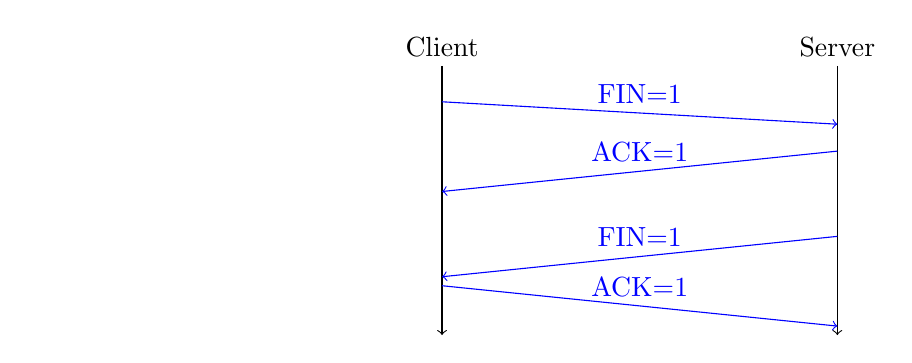
\begin{tikzpicture}
	        \begin{axis}[
	          domain=-.1:1.1,
	          xmin=-1, xmax=1.1,
	          ymin=3.8, ymax=9.8,
	          axis y line*=left,      
	          axis x line*=top,
		      x axis line style={draw=none},
		      y axis line style={draw=none},
	          height=5cm, width=1\textwidth,
	          xticklabels={Client,Server},
	          xtick={0,1},
	          tick style={draw=none},
	          yticklabels={}
	          ]
	          
			\addplot [->,black] coordinates {
				(0,9.8) (0,3.8)
			};
			\addplot [->,black] coordinates {
				(1,9.8) (1,3.8)
			};
		          
			\addplot [->,blue] coordinates {
				(0,9) (1,8.5)
			} node[above,pos=.5] {FIN=1};
			\addplot [->,blue] coordinates {
				(1,7.9) (0,7)
			} node[above,pos=.5] {ACK=1};
			
			
			\addplot [->,blue] coordinates {
				(1,6) (0,5.1) 
			} node[above,pos=.5] {FIN=1};
			\addplot [->,blue] coordinates {
				(0,4.9) (1,4)
			} node[above,pos=.5] {ACK=1};
			
		\end{axis}
    	\end{tikzpicture}
	\end{subfigure}%
\begin{subfigure}{.5\textwidth}
  \centering
	
		\includegraphics[width=7cm]{FIN-diag.png}
\end{subfigure}
\end{figure}	

\end{enumerate}



\task{3}


\begin{enumerate}[a)]


	\item \hfill
	{ \begin{center}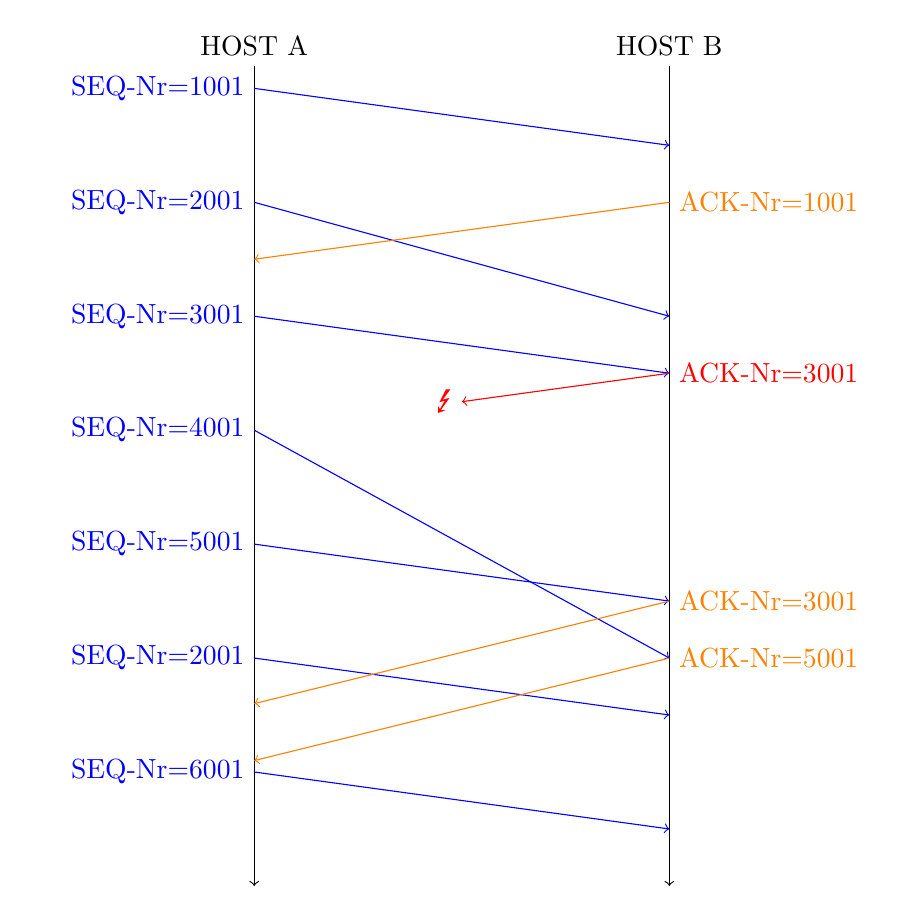
\begin{tikzpicture}
	        \begin{axis}[
	          domain=-.5:1.5,
	          xmin=-0.5, xmax=1.5,
	          ymin=0, ymax=7.2,
	          axis y line*=left,      
	          axis x line*=top,
		      x axis line style={draw=none},
		      y axis line style={draw=none},
	          height=12cm, width=1\textwidth,
	          xticklabels={HOST A,HOST B},
	          xtick={0,1},
	          tick style={draw=none},
	          yticklabels={}
	          ]
	          
			\addplot [->,black] coordinates {
				(0,7.2) (0,0)
			};
			\addplot [->,black] coordinates {
				(1,7.2) (1,0)
			};
			
			\seq{7}{1001}
			\seqt{6}{1}{2001}
			\seq{5}{3001}
			\seqt{4}{2}{4001}
			\seq{3}{5001}
			\seq{2}{2001}
			\seq{1}{6001}
			
			\ack{6}{1001}
			\ackb{4.5}{3001}
			
			\ackt{2.5}{0.9}{3001}
			\ackt{2}{0.9}{5001}

		\end{axis}
    	\end{tikzpicture}\end{center}
    }
	\item Delayed-ACK wird verwendet, um z.B. die Anzahl der Packages in Netzwerken zu verringern, wenn diese nahe ihrer Maximalkapazität sind. 
	\item Die rekursiv-definierte Formel lautet: 	$ RTT_E[k]=(1-\alpha ) \cdot RTT_E[k-1] + \alpha \cdot RTT_S[k] $ mit $RTT_E[0] = RTT_S[0] = 0$. Daraus folgt:
	
	\begin{itemize}
		\item $RTT_E[4] = (1-\alpha ) \cdot ((1-\alpha ) \cdot ((1-\alpha ) \cdot ((1-\alpha ) \cdot RTT_E[0] + \alpha \cdot RTT_S[1]) + \alpha \cdot RTT_S[2]) + \alpha \cdot RTT_S[3]) + \alpha \cdot RTT_S[4] $
		\item $RTT_E[4] \approx 2.47$
	\end{itemize}	
	

\end{enumerate}



\pointsttl{3}


\end{document}
